\documentclass{beamer}
\usepackage[utf8]{inputenc}
\usepackage[T1]{fontenc}


\title{Das neue \LaTeX-Beamer Theme der TU Dortmund}
\author{Maximilian Nöthe}
\institute[Lehrstuhl E5b \\ Fakultät Physik]{Lehrstuhl E5b \par\vspace{3pt} Fakultät Physik}
\titlegraphic{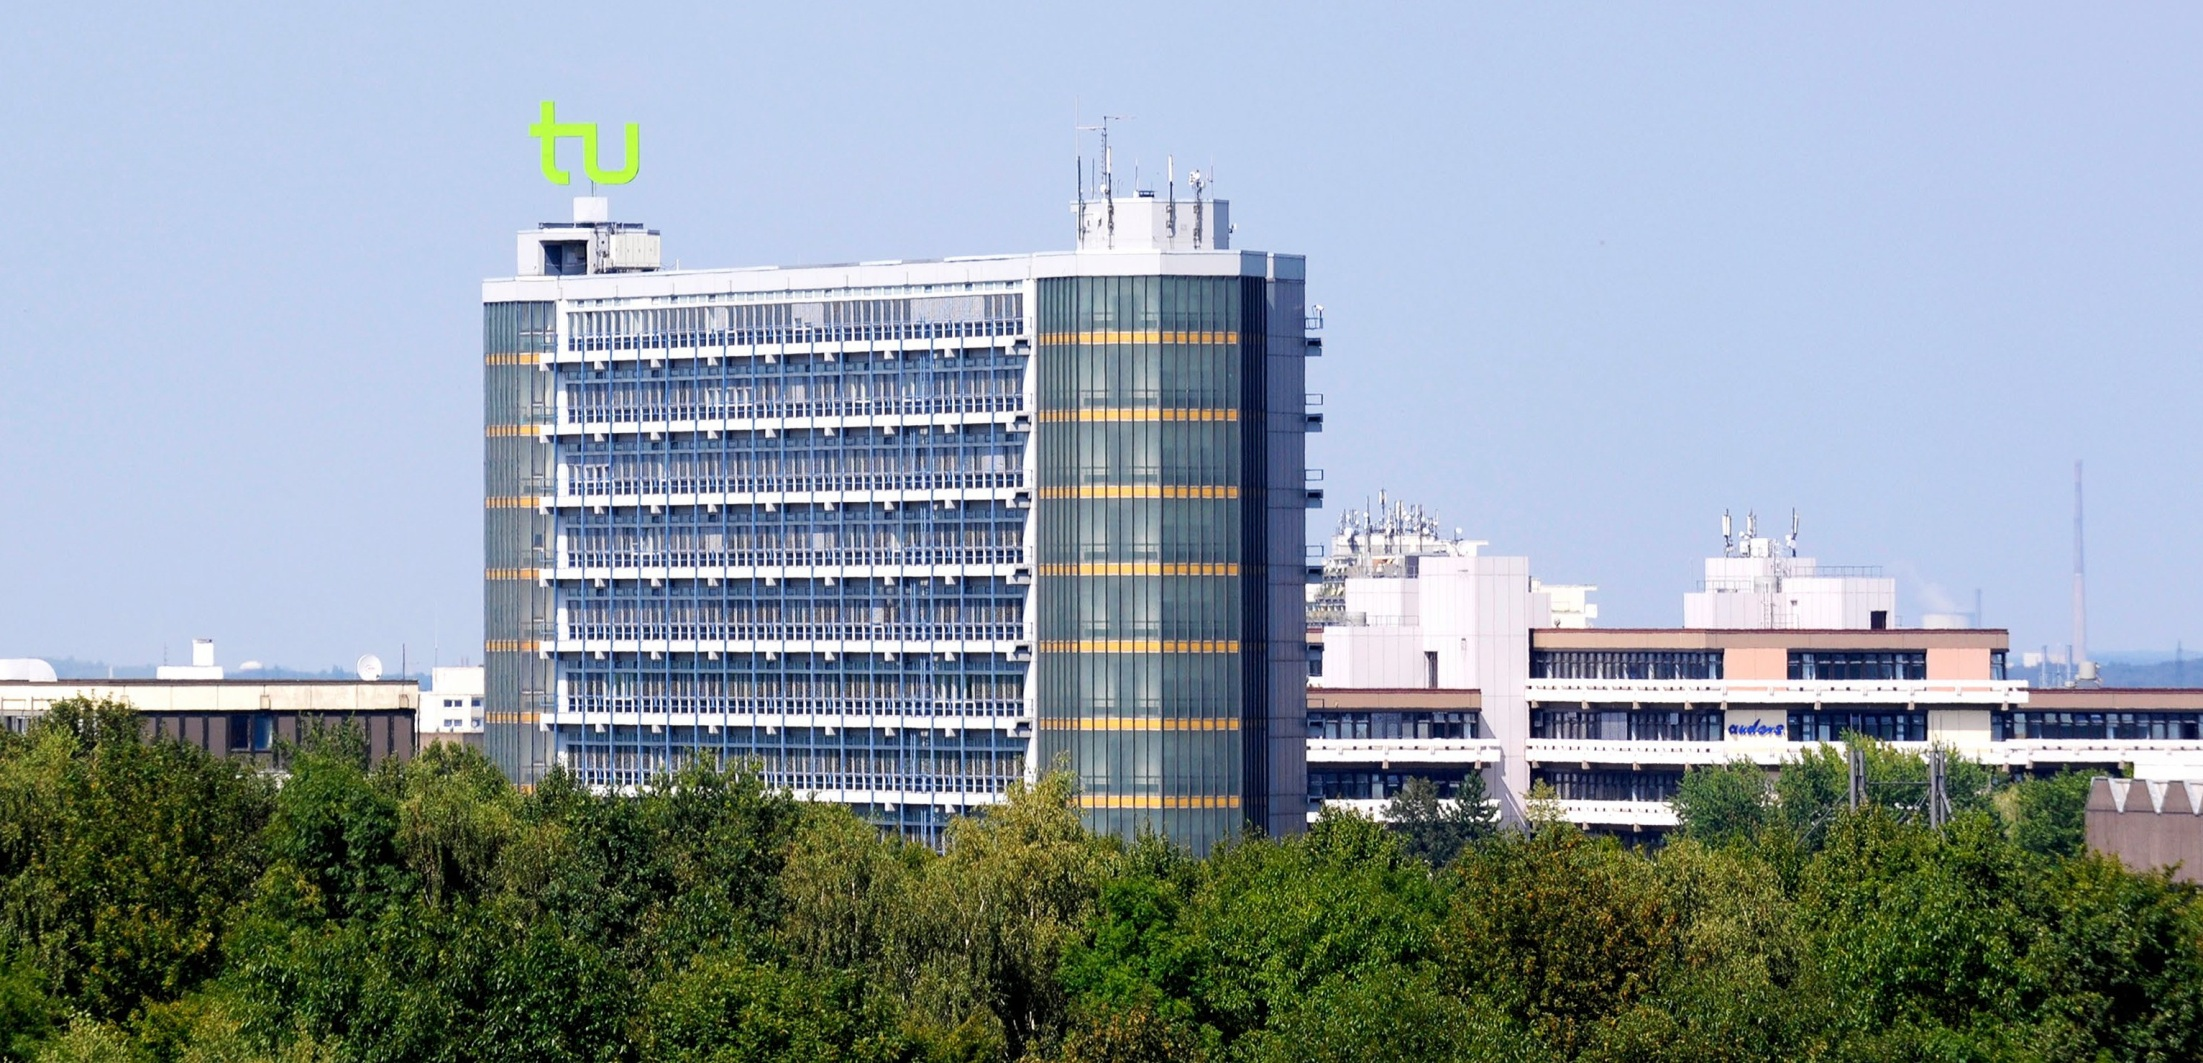
\includegraphics[height=0.7\textheight]{Title-Pic.jpg}}

\usetheme{TUDo}

\begin{document}

\begin{frame}
\setcounter{framenumber}{0}
    \titlepage
\end{frame}

\begin{frame}
    \frametitle{Einführung}
    \tableofcontents[pausesections]
\end{frame}

\section{Das Design}
\subsection{Farben}
\begin{frame}
    \frametitle{Die TU-Farbpalette}
    \begin{itemize}
        \item \textcolor{TUgreen}{TUgreen}
            \begin{itemize}
                \item \textcolor{TUlightgreen}{TUlightgreen}
                \item \textcolor{TUdarkgreen}{TUdarkgreen}
                \item \textcolor{TUolive}{TUolive}
            \end{itemize}
        \item \textcolor{TUyellow}{TUyellow}
        \item \textcolor{TUcitron}{TUcitron}
        \item \textcolor{TUlime}{TUlime}
        \item \textcolor{TUorange}{TUorange}
    \end{itemize}
\end{frame}

\subsection{Blöcke}
\begin{frame}
    \frametitle{Blöcke}
    \begin{block}{block}
        \begin{itemize}
            \item Standardblock
            \item gedacht für normalen, strukturierten Text
        \end{itemize}
    \end{block}
    \begin{alertblock}{alertblock}
        \begin{itemize}
            \item Block in auffallnderer Farbe 
        \end{itemize}
    \end{alertblock}
    \begin{exampleblock}{exampleblock}
        \begin{itemize}
            \item Noch ein anderer Block
        \end{itemize}
    \end{exampleblock}
\end{frame}

\section{Beispiel-Slides}
\subsection{Zweispaltige Layouts}
\begin{frame}
    \frametitle{Zwei Columns für Text}
    \begin{columns}[t]
        \begin{column}{0.5\textwidth}
            \begin{itemize}[<+->]
            \item Toller Punkt
            \item zweiter Toller Punkt
        \end{itemize}
        \end{column}
        \begin{column}{0.5\textwidth}
            \begin{enumerate}
                \item Punkt
                \item Punkt
                \item Punkt
            \end{enumerate}
        \end{column}
    \end{columns}
\end{frame}

\begin{frame}
    \frametitle{Je eine Column für Text/Bild}
    % Für Bilder Argument T benutzen:
    \begin{columns}[T]
        \begin{column}{0.5\textwidth}
            \begin{itemize}[<+->]
            \item super Mathe-Tower
            \item super TU-Logo
            \item super Bild
            \item super geil
        \end{itemize}
        \end{column}
        \begin{column}{0.5\textwidth}
            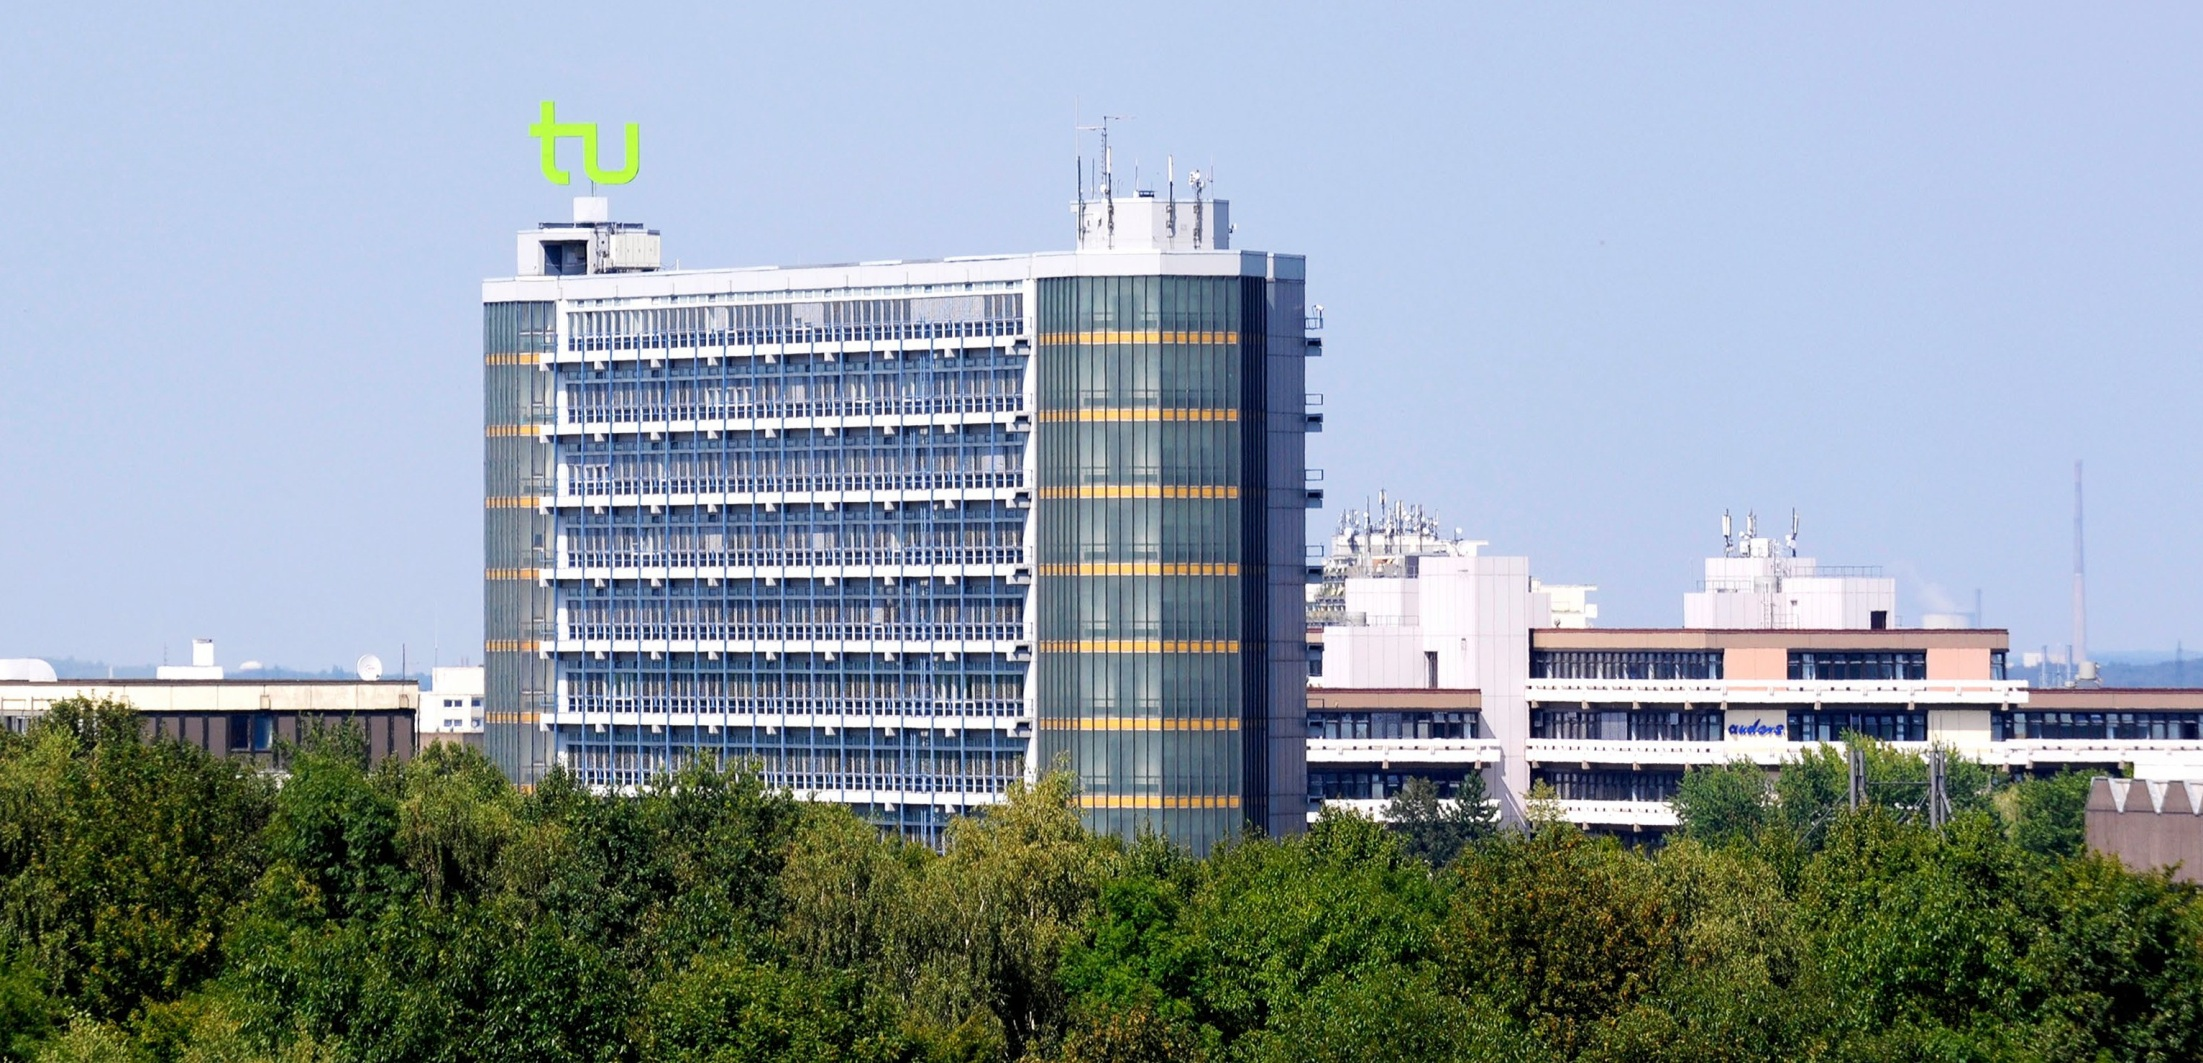
\includegraphics[width=\textwidth]{./Title-Pic.jpg}
        \end{column}
    \end{columns}
\end{frame}
\begin{frame}
    \frametitle{2x2 Columns für Bild/Text}
    % Für Bilder Argument T benutzen:
    \begin{columns}[T]
        \begin{column}{0.5\textwidth}
            \begin{itemize}%[<+->] Kommentar entfernen falls jeder Punkt einzeln erscheinen soll
            \item super Mathe-Tower
            \item super TU-Logo
            \item super Bild
            \item super geil
        \end{itemize}
        \end{column}
        \begin{column}{0.5\textwidth}
            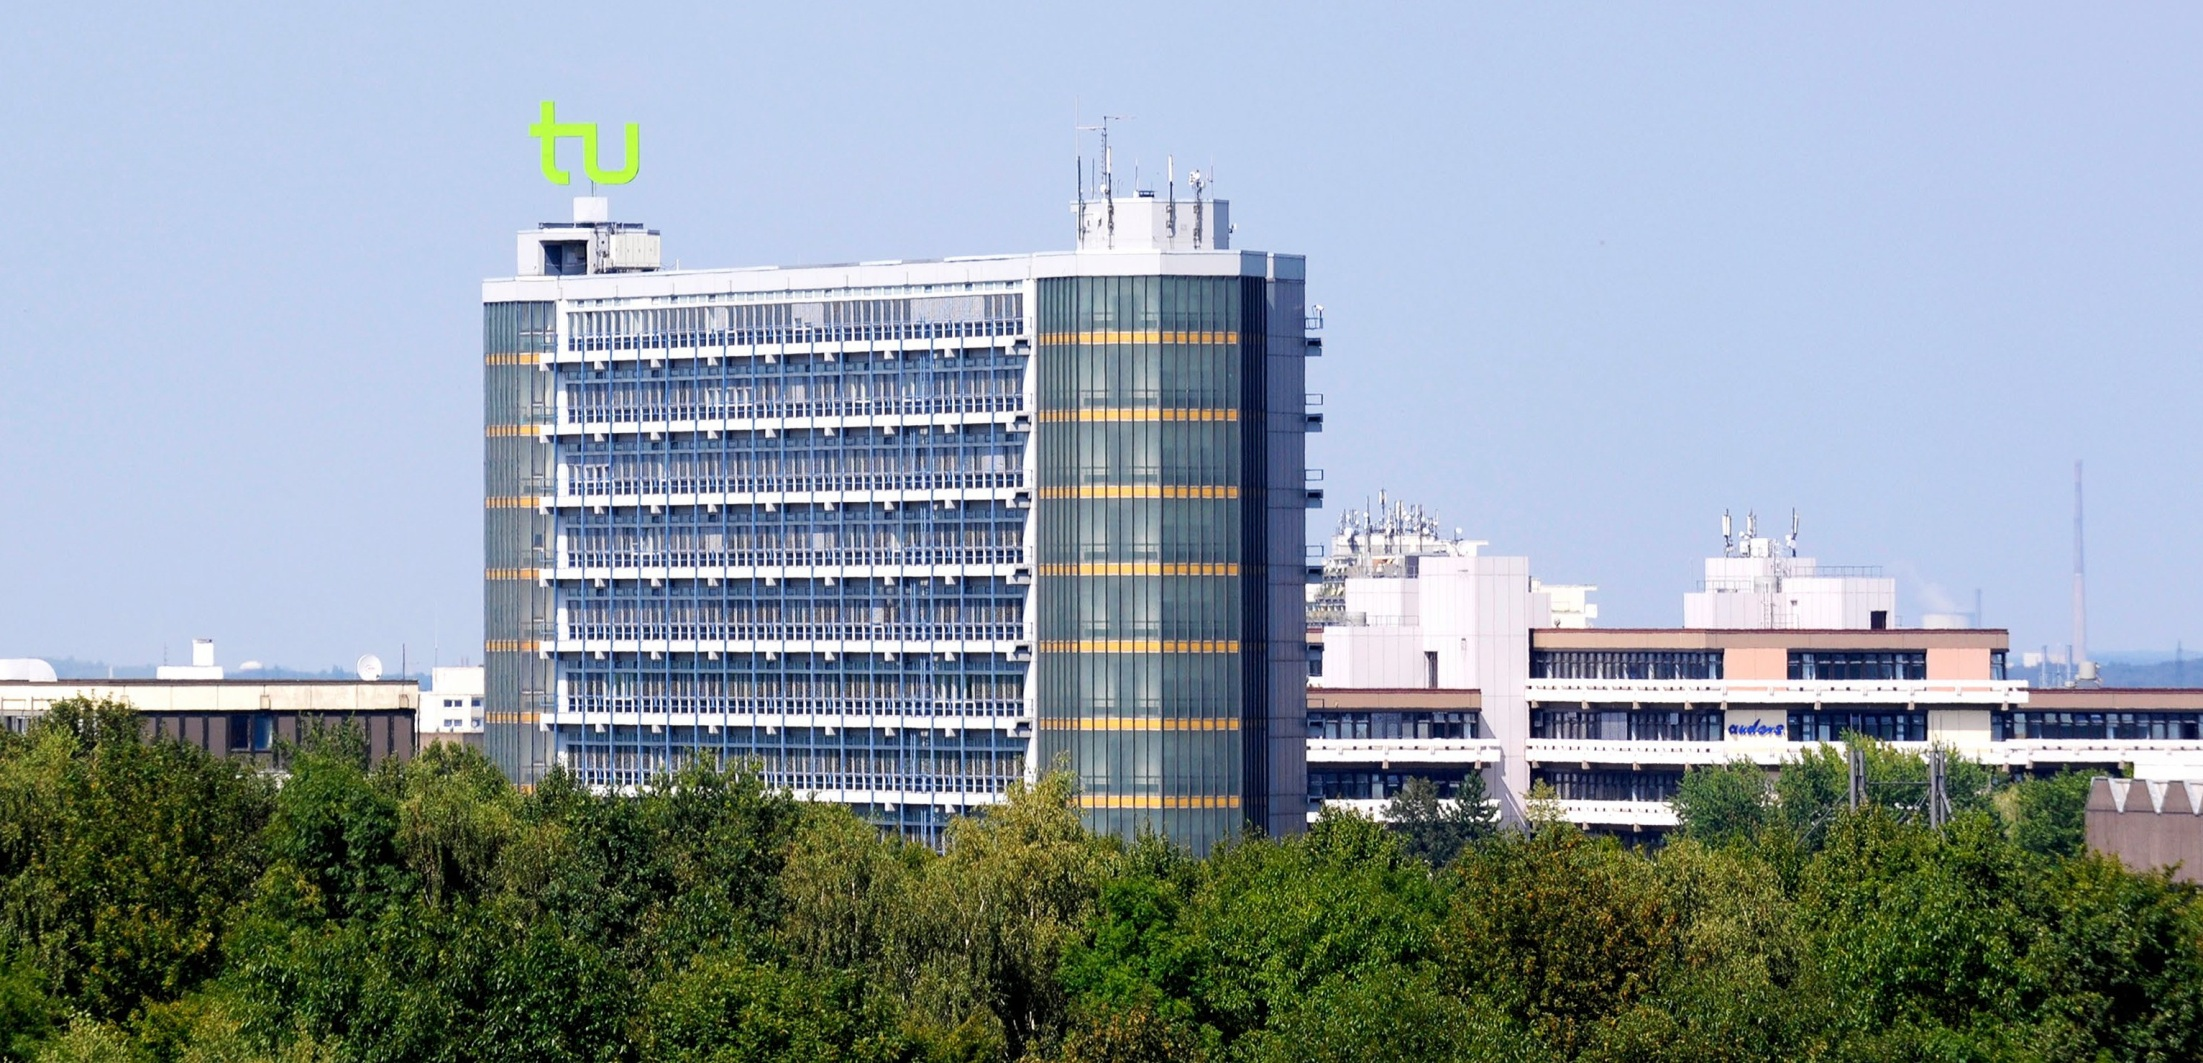
\includegraphics[width=\textwidth]{./Title-Pic.jpg}
        \end{column}
    \end{columns}
\end{frame}
\begin{frame}
    \frametitle{2x2 Columns für Bild/Text}
    % Für Bilder Argument T benutzen:
    \begin{columns}[T]
        \begin{column}{0.5\textwidth}
            \begin{itemize}%[<+->] Kommentar entfernen falls jeder Punkt einzeln erscheinen soll
                \item super Mathe-Tower
                \item super TU-Logo
                \item super Bild
                \item super geil
            \end{itemize}
        \end{column}
        \begin{column}{0.5\textwidth}
            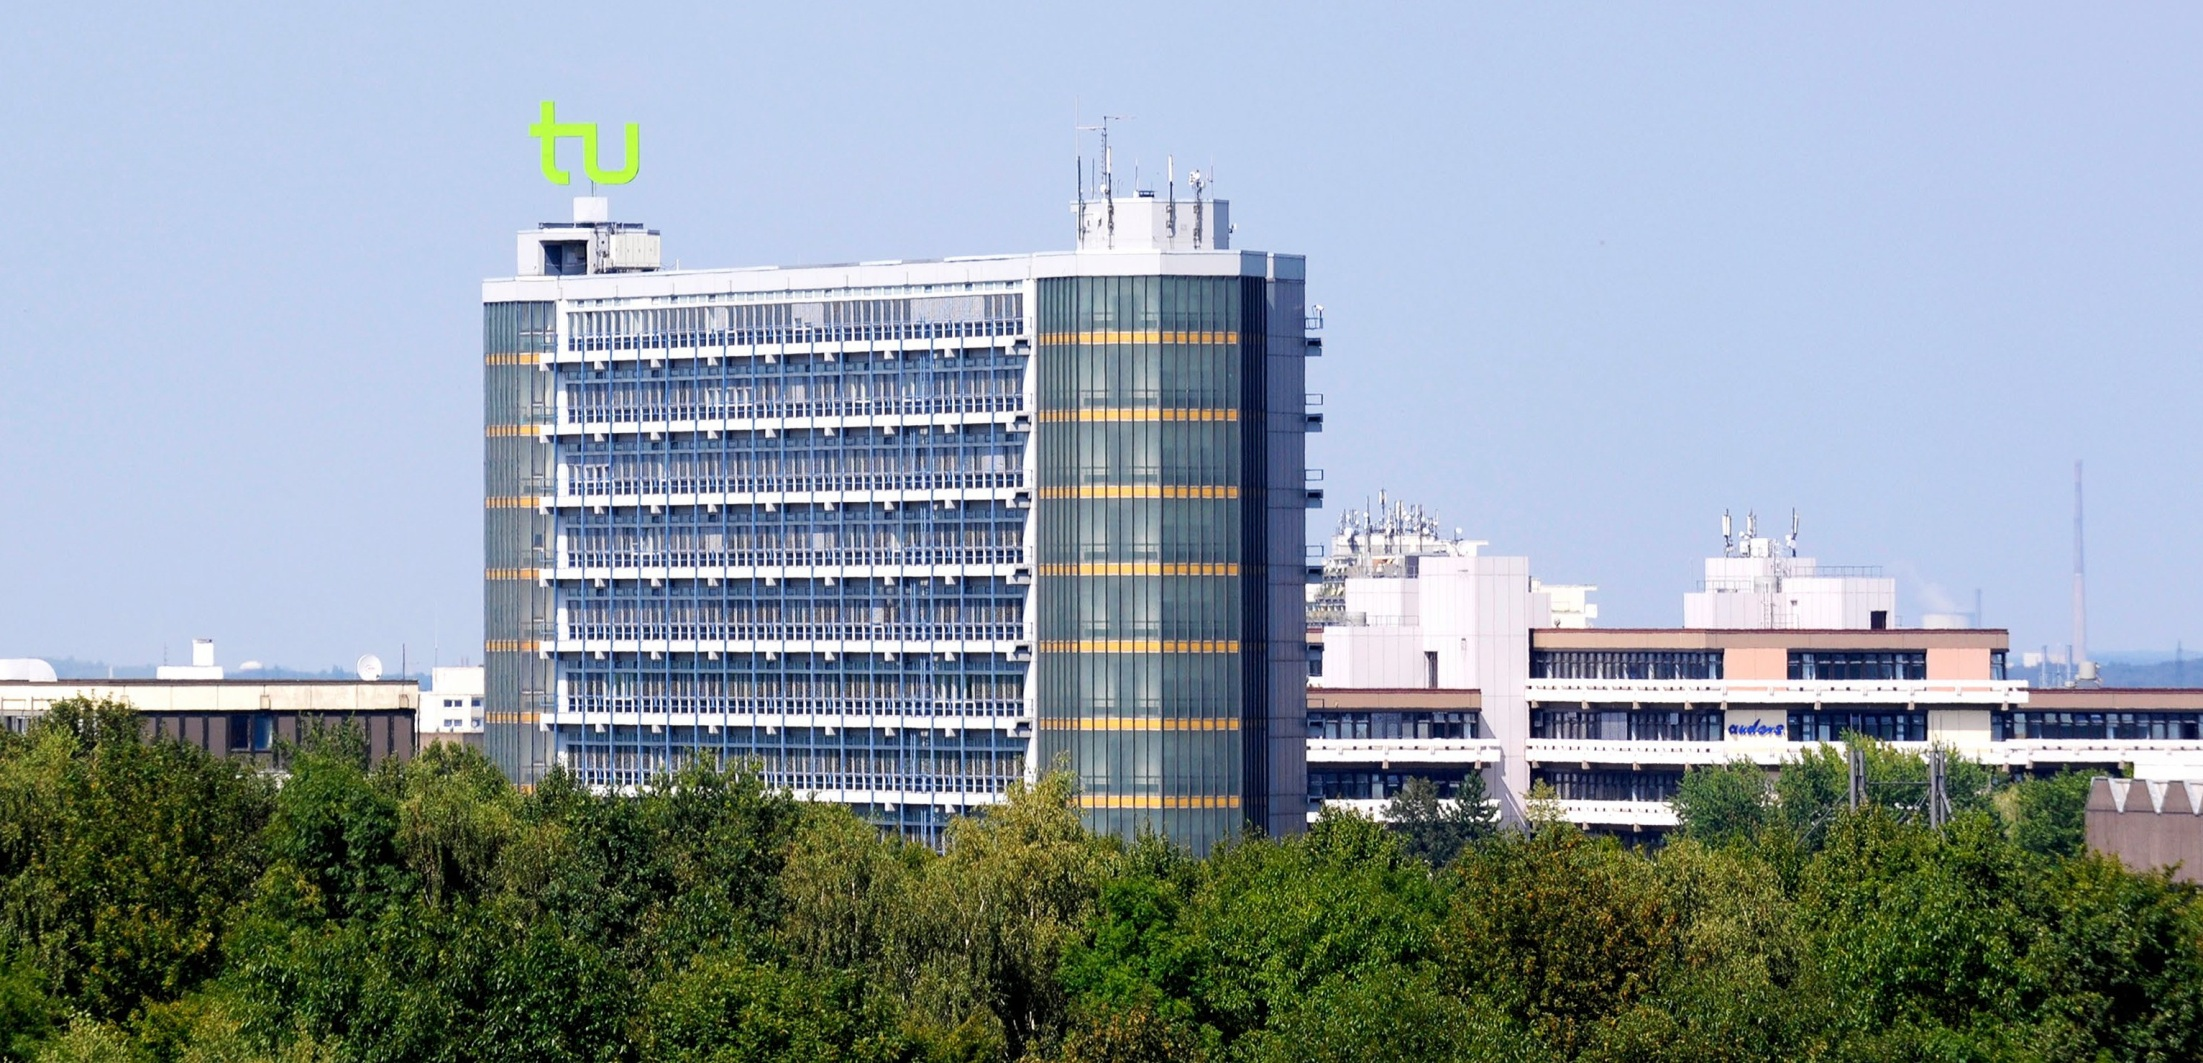
\includegraphics[width=\textwidth]{./Title-Pic.jpg}
        \end{column}
    \end{columns}
    \vspace{5pt}
    \begin{columns}[T]
        \begin{column}{0.5\textwidth}
            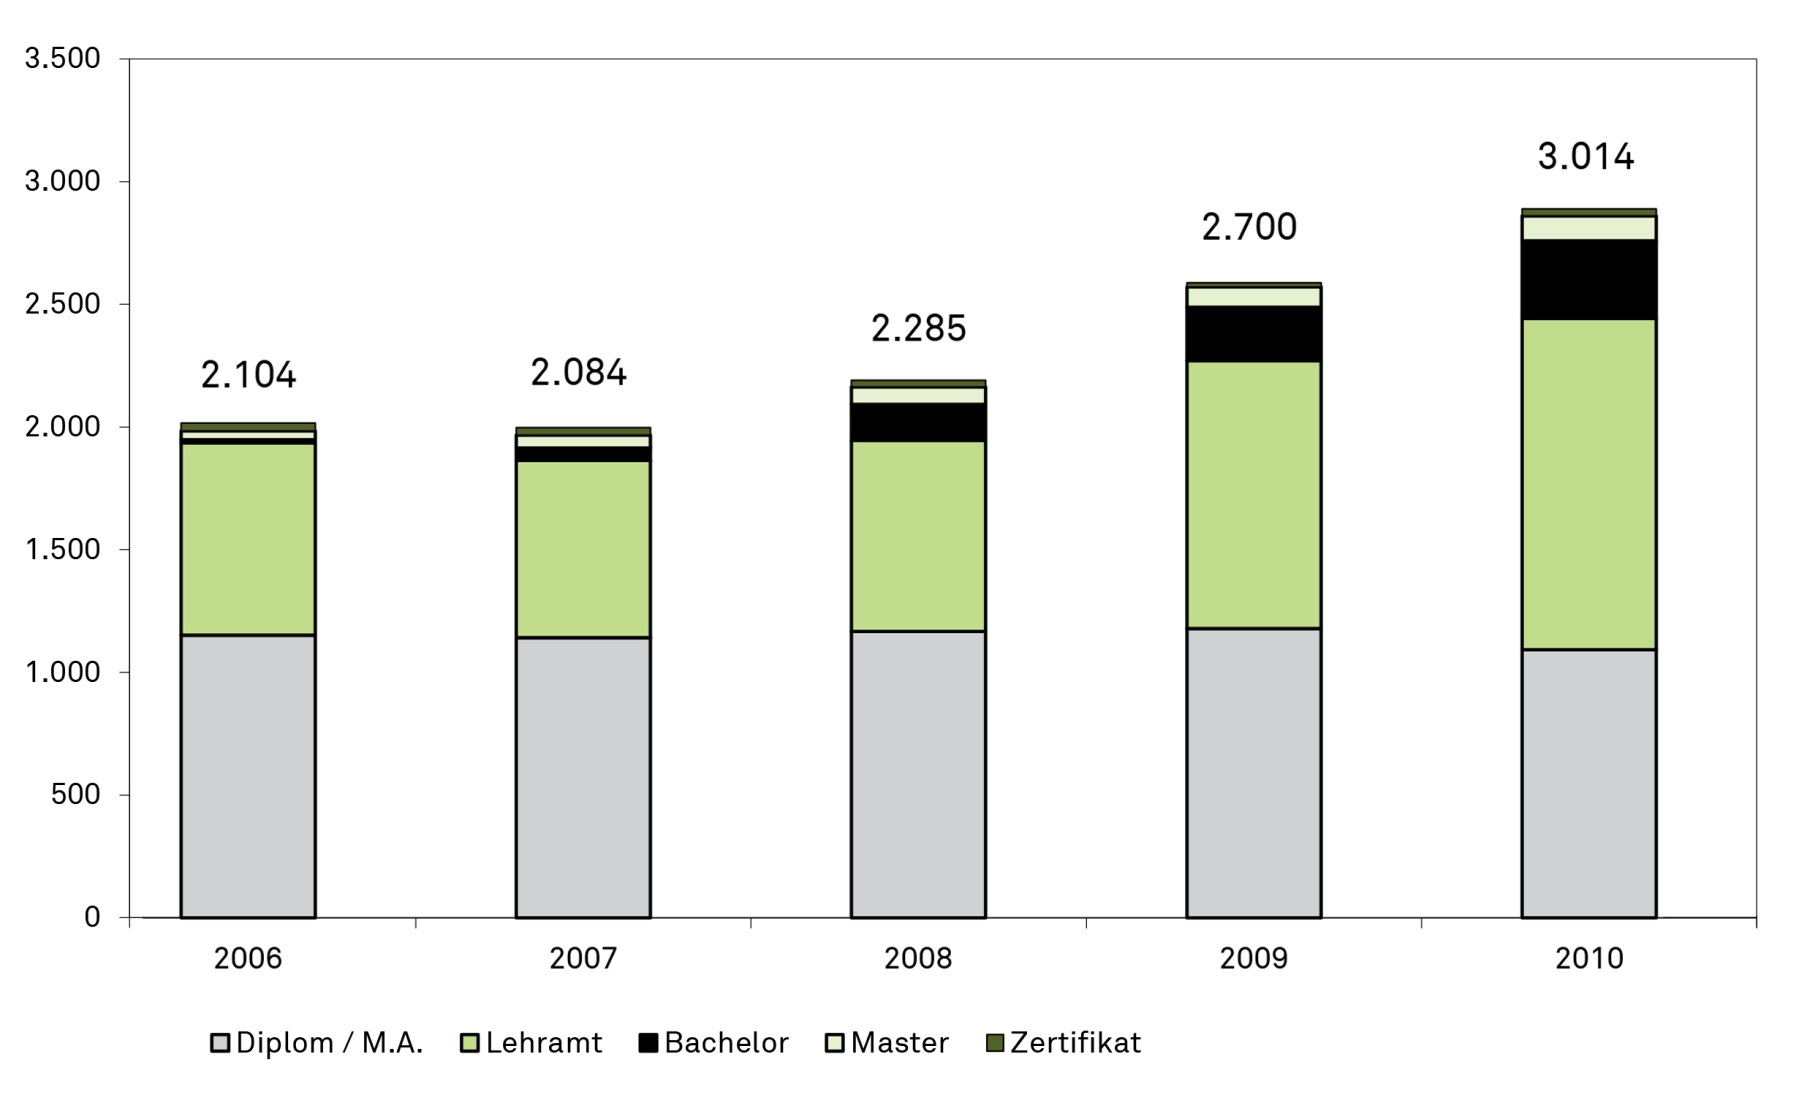
\includegraphics[width=\textwidth]{./image23.jpg}
        \end{column}
        \begin{column}{0.5\textwidth}
            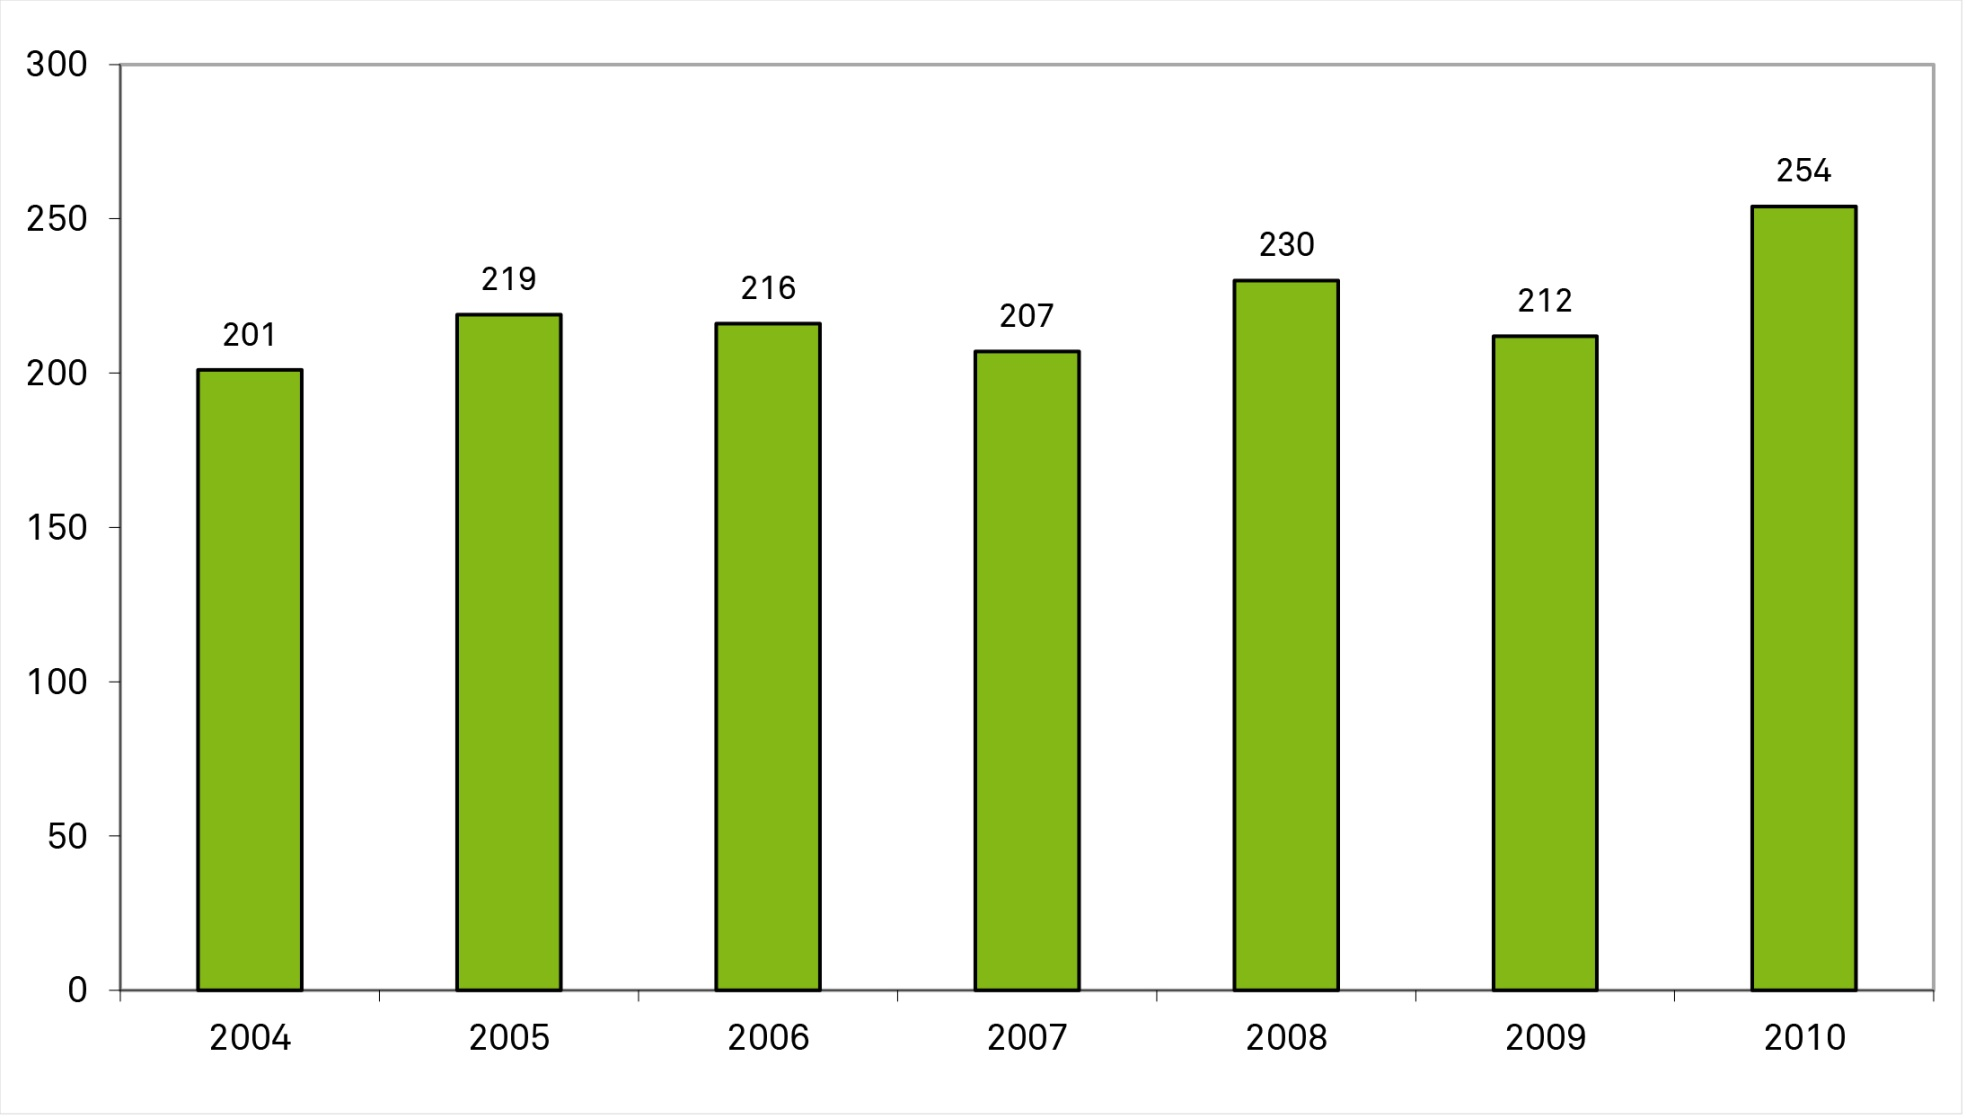
\includegraphics[width=\textwidth]{./image24.jpg}
        \end{column}
    \end{columns}
\end{frame}
\end{document}
